\documentclass[12pt, a4paper, oneside]{article}
\usepackage{graphicx}
\usepackage{arial}
\renewcommand{\familydefault}{\sfdefault}
\usepackage[T1]{fontenc}
\usepackage[polish]{babel}
\usepackage[utf8]{inputenc}
\usepackage{lmodern}
\usepackage[left=2cm,right=2cm,top=2cm,bottom=2cm]{geometry}
\selectlanguage{polish}

\begin{document}
\pagenumbering{gobble}
\begin{figure}[h]
\centering
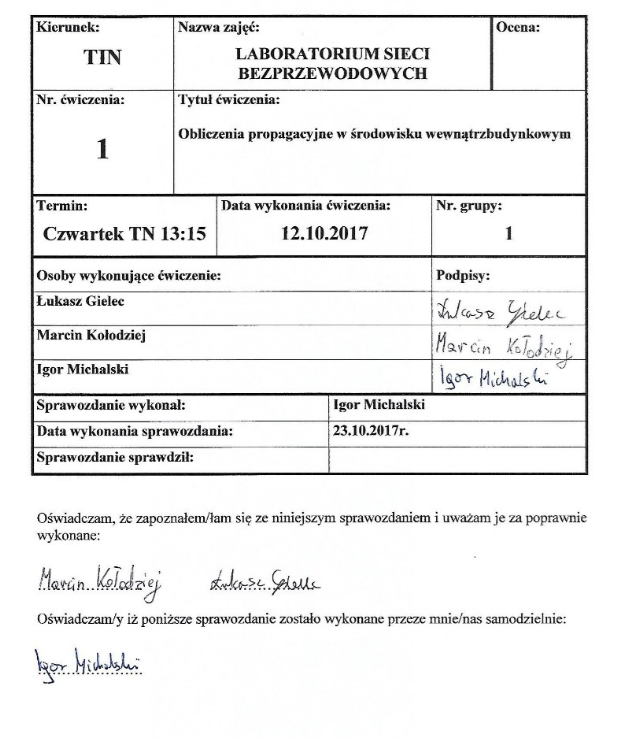
\includegraphics[scale=0.8]{title_page.png}
\end{figure}
\clearpage
\pagenumbering{arabic}
\section{Wstęp}
\indent\indent Obliczenia propagacyjne mają na celu wyznaczenie rozkładu natężenia pola na danym obszarze. Podczas laboratorium wykonywane są symulacje dla trzech wewnątrzbudynkowych modeli propagacyjnych: Dominant-Path (DPM), Multi-Wall (MWM), One-Slope (OSM). Całkowite tłumienie pomiędzy nadajnikiem i odbiornikiem opisywane jest dla kolejnych modeli wzorami:
\begin{equation}
L=20\cdot p\cdot log_{10}(d)+\sum_{i=1}^nf(\phi,i)+\sum_{j=1}^mL_j-\alpha,
\end{equation}
gdzie:
\begin{itemize}
\item $p$ - współczynnik tłumienia trasy zależny od otoczenia,
\item $d~[m]$ - odległość między nadajnikiem i odbiornikiem,
\item $f(\phi,i)~[dB]$ - funkcja opisująca tłumienie związane ze zmianą kierunku rozchodzenia fali,
\item $L_j~[dB]$ - tłumienie j-tej ściany,
\item $\alpha~[dB]$ - współczynnik falowodowy (np. zysk podczas propagacji w korytarzach, gdzie zachodzi efekt falowodowy).
\end{itemize}
\begin{equation}
L=L_{fs}(d)+L_c+\sum_{i=1}^Ik_{wi}\cdot L_{wi}+k_f^{[\frac{k_f+2}{k_f+1}-b]}\cdot L_f,
\end{equation}
gdzie:
\begin{itemize}
\item $L_{fs}~[dB]$ - tłumienie wolnej przestrzeni pomiędzy nadajnikiem i odbiornikiem,
\item $L_c~[dB]$ - stałe tłumienie (często bliskie zeru),
\item $k_{wi}$ - ilość ścian i-tego typu na trasie propagacji,
\item $L_{wi}~[dB]$ - tłumienie ściany i-tego typu,
\item $k_f$ - ilość stropów na trasie propagacji,
\item $L_f~[dB]$ - tłumienie pomiędzy sąsiadującymi piętrami,
\item $b$ - parametr empiryczny.
\end{itemize}
\begin{equation}
L=L_0+10\cdot n\cdot log_{10}(d),
\end{equation}
gdzie:
\begin{itemize}
\item $L_0~[dB]$ - tłumienie wolnej przestrzeni w odległości 1m od nadajnika,
\item $n$ - współczynnik zaniku,
\item $d~[m]$ - odległość między nadajnikiem i odbiornikiem,
\end{itemize}
DPM oraz MWM są modelami dokładniejszymi - biorą pod uwagę więcej czynników, które wpływają na tłumienie trasy radiowej. OSM jest modelem znacznie prostszym, mniej dokładnym i wymaga oszacowania współczynnika zaniku dla danego obszaru.
\clearpage
\noindent Tabela 1: Tłumienie poszczególnych elementów w środowisku wewnątrzbudynkowym,\\w paśmie 2.4 GHz
\begin{figure}[h]
\centering
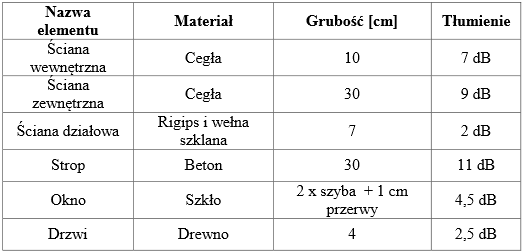
\includegraphics[scale=0.7]{tab1.png}
\end{figure}
\section{Stosowane wzory}
\indent\indent Ponieważ obliczenia dotyczą wyłącznie jednego piętra, wzór dla MWM został uproszczony o~człon wnoszący poprawki dla tras propagacji biegnących przez stropy. Wykorzystano go w poniższej formie.
\begin{equation}
L=L_{fs}+L_c+\sum_{i=1}^Ik_{wi}L_{wi}
\end{equation}
\indent\indent Opisuje on całkowitą tłumienność trasy jako sumę trzech składowych - tłumienie wolnej przestrzeni $L_{fs}$, stałe tłumienie $L_c$ oraz sumę składającą się z iloczynów współczynnika tłumienia ściany $L_{wi}$~oraz liczby $k_{wi}$~ścian danego typu na trasie propagacji. Tłumienie wolnej przestrzeni jako funkcja odległości oraz częstotliwości opisywane jest wzorem (5).
\begin{equation}
L_{fs}=-27.55+20\cdot log_{10}(f~[MHz])+20\cdot log_{10}(d~[m])
\end{equation}
\indent\indent Do obliczenia modelu OS wykorzystany został wzór (3).
\section{Przykładowe obliczenia}
\subsection{Multi-Wall Model}
\indent\indent Do obliczeń przyjęte zostały:
\begin{itemize}
\item $P_N=20~dBm$
\item $f=2472~MHz$
\item $k_{w1}=4$
\item $L_{w1}=6.9~dB$
\item $d=17~m$
\item $L_c=0~dB$
\end{itemize}
\indent\indent Pierwszym krokiem jest obliczenie tłumienia wolnej przestrzeni:
\begin{equation}
L_{fs}=-27.55+20\cdot log_{10}(2472)+20\cdot log_{10}(17)=64.92~[dB]
\end{equation}
\indent Następnie należy wykorzystać tę wartość do obliczenia całkowitego tłumienia trasy:
\begin{equation}
L=64.92+0+5\cdot6.9=99.42~[dB]
\end{equation}
\indent W porównaniu z wynikami symulacji okazuje się, że wartości są znacząco różne. W powyższych obliczeniach należy uwzględnić także szafy stojące na drodze. Można założyć, że każda z nich, w przybliżeniu, posiada tłumienie jak 1.5 drewnianych drzwi o grubości 4 cm. W~tym wypadku powstają nowe współczynniki $k_{w2}=4$ oraz $L_{w2}=3.75~dB$.
\begin{equation}
L=99.42+4\cdot 3.75 = 114.42~[dB]
\end{equation}
\indent\indent Jest to wynik zaledwie o 0.8 dB większy od wartości wyznaczonej podczas symulacji dla tego samego punktu.
\subsection{One-Slope Model}
\indent\indent Do obliczeń przyjęte zostały:
\begin{itemize}
\item $n=6$
\item $d=10~m$
\end{itemize}
\indent\indent Pierwszym krokiem ponownie jest obliczenie tłumienia wolnej przestrzeni w odległości 1 m od nadajnika:
\begin{equation}
L_0=-27.55+20\cdot log_{10}(2472)+20\cdot log_{10}(1)=40.31~[dB]
\end{equation}
\indent Następnie należy wykorzystać tę wartość do obliczenia całkowitego tłumienia trasy:
\begin{equation}
L=40.31+60\cdot log_{10}(10)=100.31~[dB]
\end{equation}
\section{Przebieg ćwiczenia}
\indent\indent Po zgłoszeniu gotowości i uruchomieniu przez prowadzącego odpowiedniego oprogramowania, można było przystąpić do wykonywania ćwiczenia. Zgodnie z instrukcją stworzony został nowy projekt bazujący na modelu ósmego piętra budynku C-5. Wczytane zostały predefiniowane ustawienia interfejsu radiowego zgodnego z IEEE 802.11g. W prawym, górnym rogu modelu umieszczony został punkt dostępowy. Przyjęto EIRP = 20 dBm oraz kanał nr 13 (częstotliwość środkowa 2472 MHz).\\
\indent Wykonane zostały symulacje dla DPM, MWM, po czym nastąpiła awaria programu (zawiesił się). Po ponownym uruchomieniu umieszczono punkt dostępowy w tym samym miejscu i przeprowadzono symulację dla modelu OSM.\\
\indent Do wszystkich obliczeń przyjęto rozdzielczość 0.1 m. Zapisano wyniki symulacji w postaci mapek rozkładów mocy, mapek szybkości transmisji oraz rozkładów mocy i szybkości transmisji dla dwóch ścieżek (zgodnych z instrukcją).\\
\indent Następnie utworzono nowy projekt i dodano dwa punkty dostępowe o EIRP 20 dBm, pracujące na kanałach nr 1 (częstotliwość środkowa 2412 MHz) oraz nr 13. Oba punkty dostępowe zostały rozmieszczone metodą prób i~błędów tak, aby uzyskać jak najlepsze parametry transmisji na poziomie całego piętra. Parametry wyznaczone zostały z wykorzystaniem MWM.
\clearpage
\section{Wyniki symulacji}
\subsection{Mapki rozkładów mocy}
\begin{figure}[h]
\centering
\caption{Rozkład mocy - Multi-Wall Model}
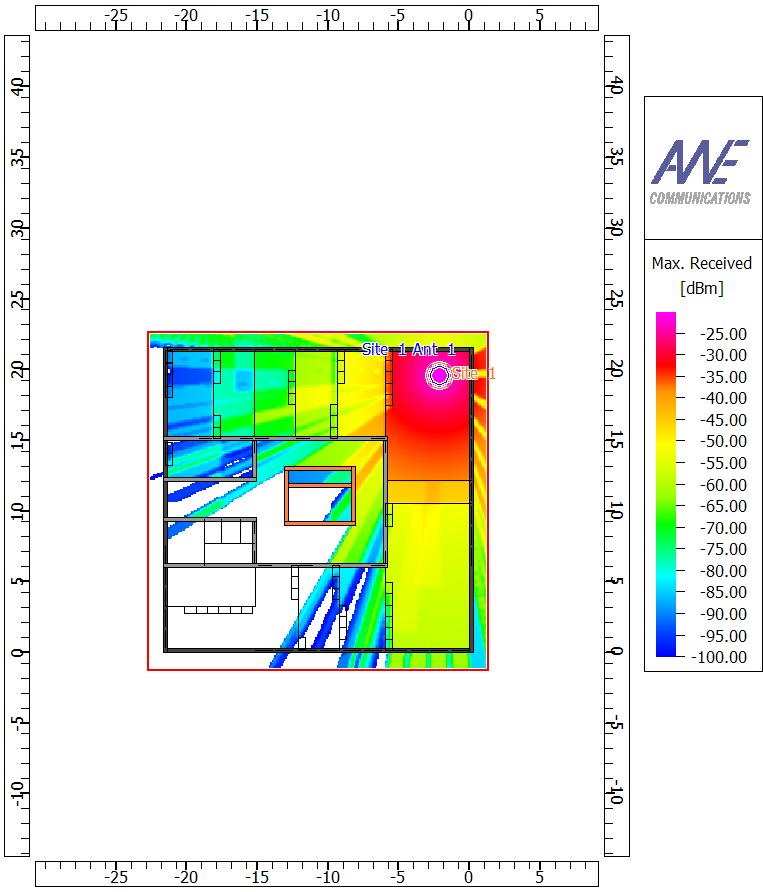
\includegraphics[scale=0.62]{MWM_RECEIVED.png}
\end{figure}
\begin{figure}[h]
\centering
\caption{Rozkład mocy - Dominant-Path Model}
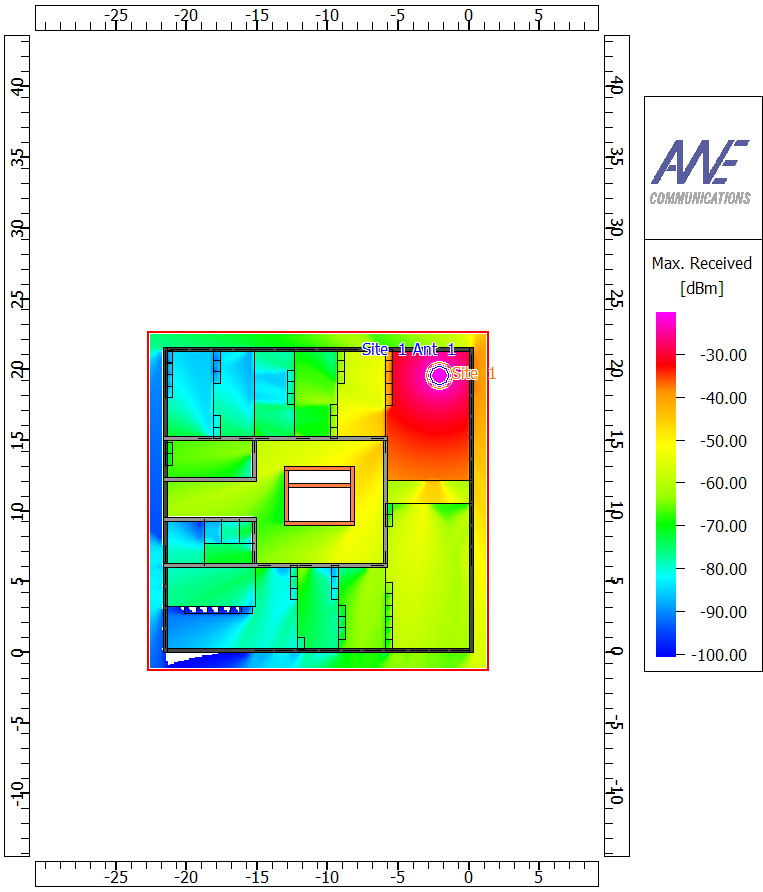
\includegraphics[scale=0.65]{DPM_RECEIVED.png}
\end{figure}
\begin{figure}[h]
\centering
\caption{Rozkład mocy - One-Slope Model ze współczynnikiem n = 2}
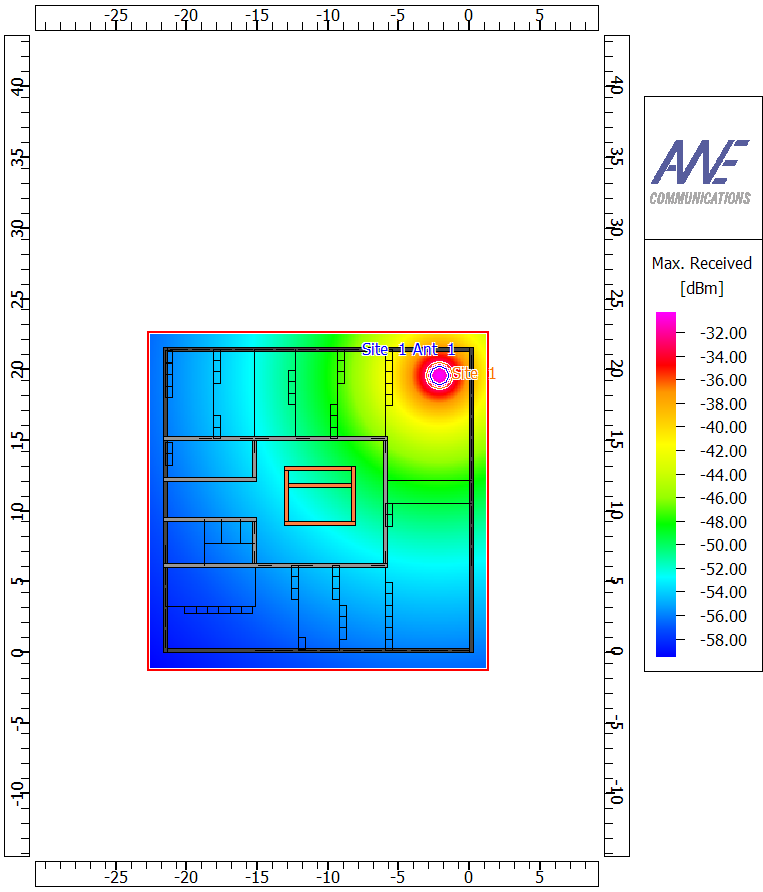
\includegraphics[scale=0.65]{ONE_SLOPE_RECEIVED_EXP_2.png}
\end{figure}
\begin{figure}[h]
\centering
\caption{Rozkład mocy - One-Slope Model ze współczynnikiem n = 6}
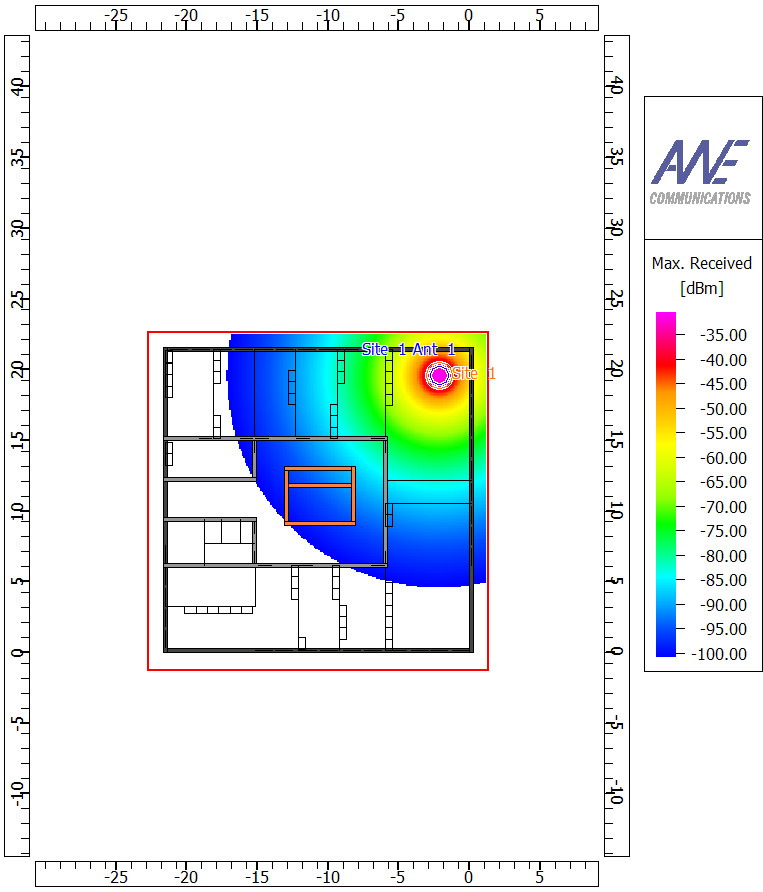
\includegraphics[scale=0.65]{ONE_SLOPE_RECEIVED_EXP_6.png}
\end{figure}
\clearpage
\subsection{Mapki szybkości transmisji}
\begin{figure}[h]
\centering
\caption{Szybkość transmisji - Multi-Wall Model}
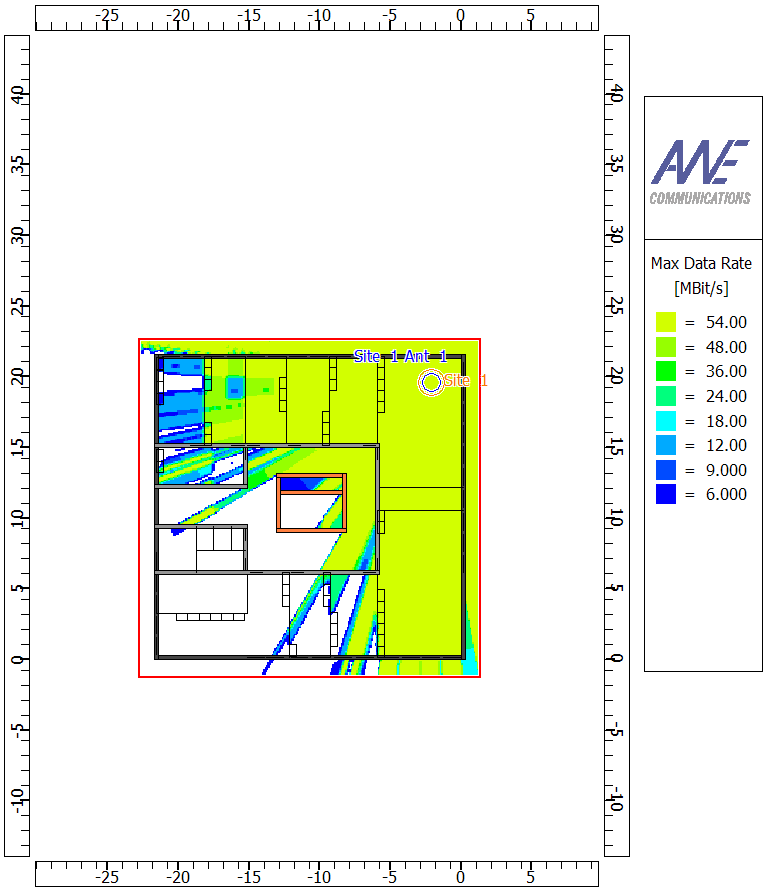
\includegraphics[scale=0.63]{MWM_RATE.png}
\end{figure}
\begin{figure}[h]
\centering
\caption{Szybkość transmisji - Dominant-Path Model}
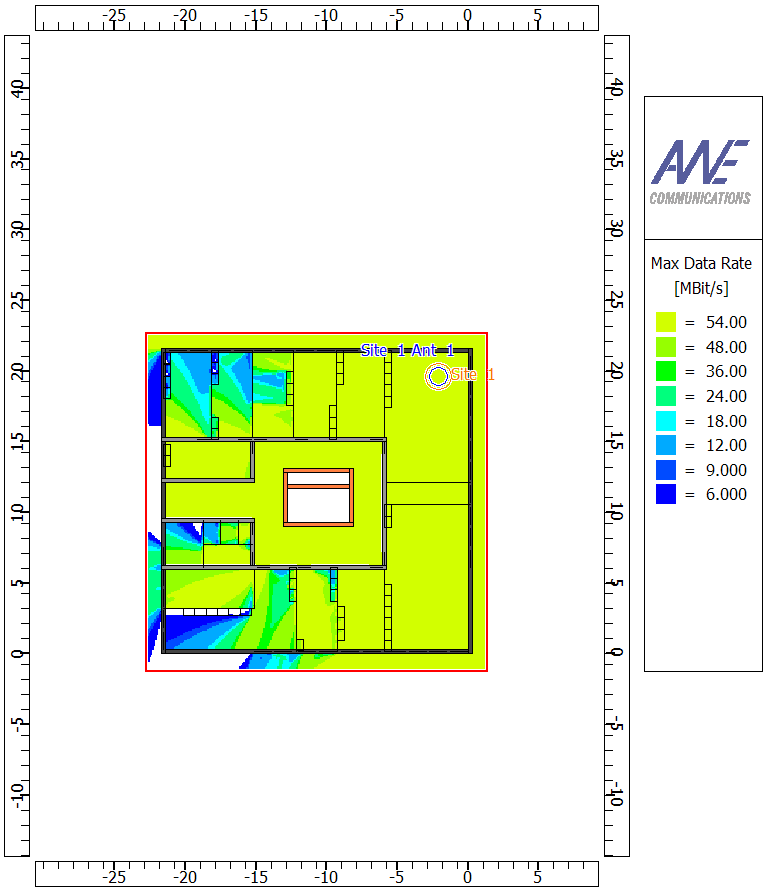
\includegraphics[scale=0.65]{DPM_RATE.png}
\end{figure}
\begin{figure}[h]
\centering
\caption{Szybkość transmisji - One-Slope Model ze współczynnikiem n = 2}
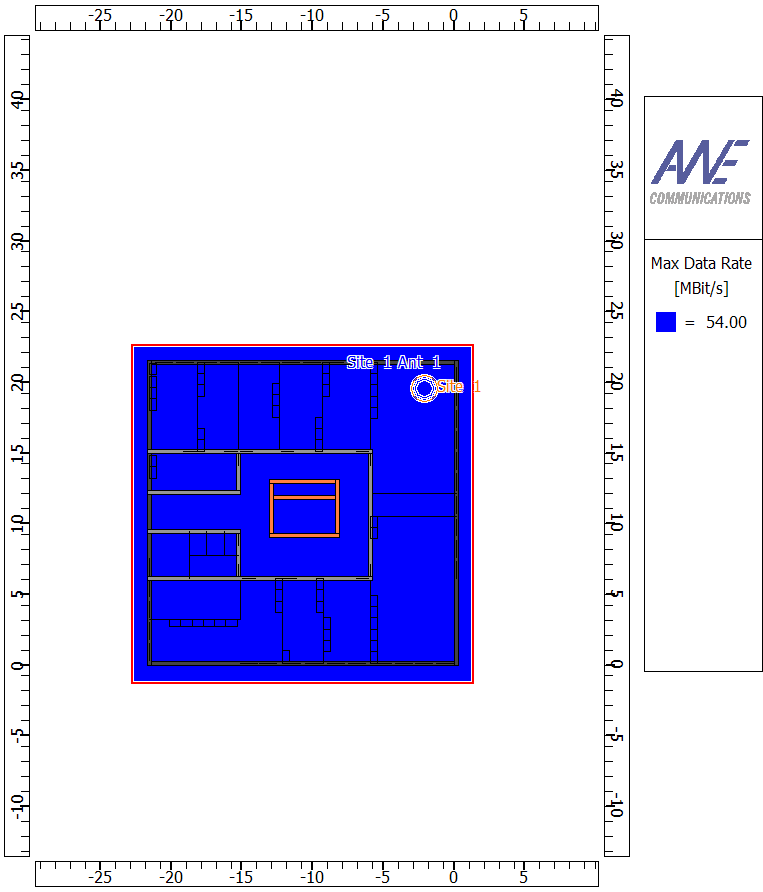
\includegraphics[scale=0.65]{ONE_SLOPE_RATE_EXP_2.png}
\end{figure}
\begin{figure}[h]
\centering
\caption{Szybkość transmisji - One-Slope Model ze współczynnikiem n = 6}
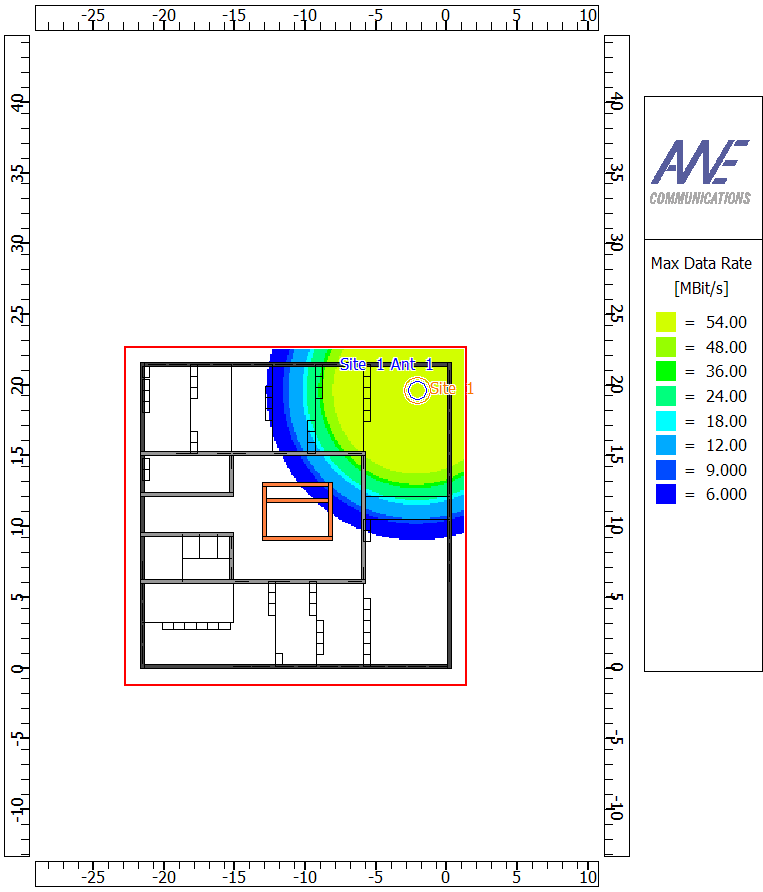
\includegraphics[scale=0.65]{ONE_SLOPE_RATE_EXP_6.png}
\end{figure}
\clearpage
\subsection{Mapki rozkładów mocy oraz szybkości transmisji dla dwóch nadajników pracujących na częstotliwościach odległych o 12 kanałów}
\begin{figure}[h]
\centering
\caption{Rozkład mocy - Multi-Wall Model}
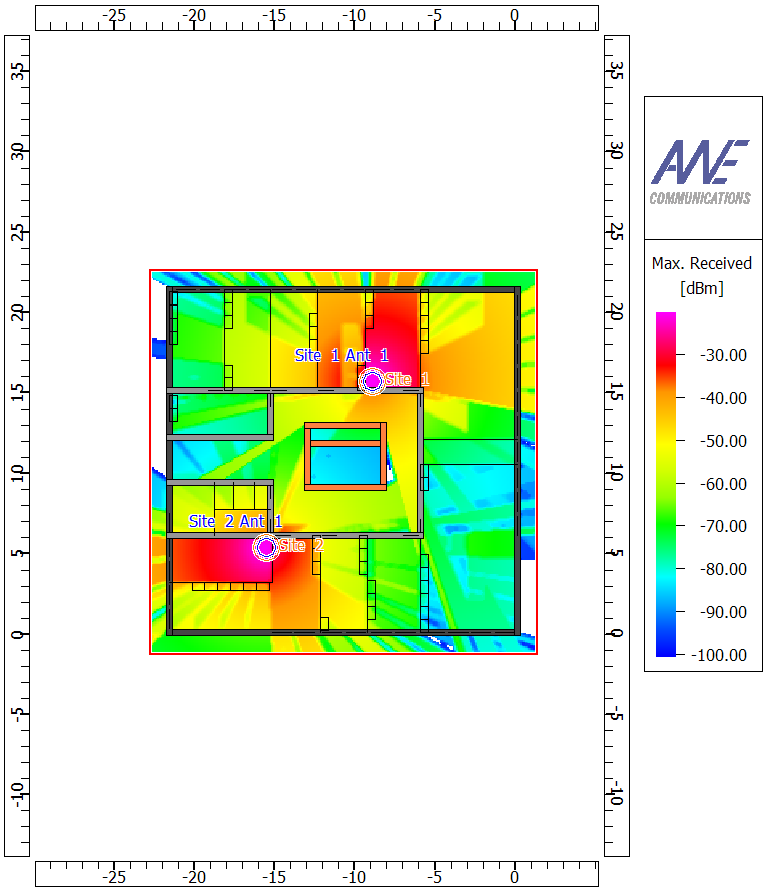
\includegraphics[scale=0.63]{RECEIVED.png}
\end{figure}
\begin{figure}[h]
\centering
\caption{Szybkość transmisji - Multi-Wall Model}
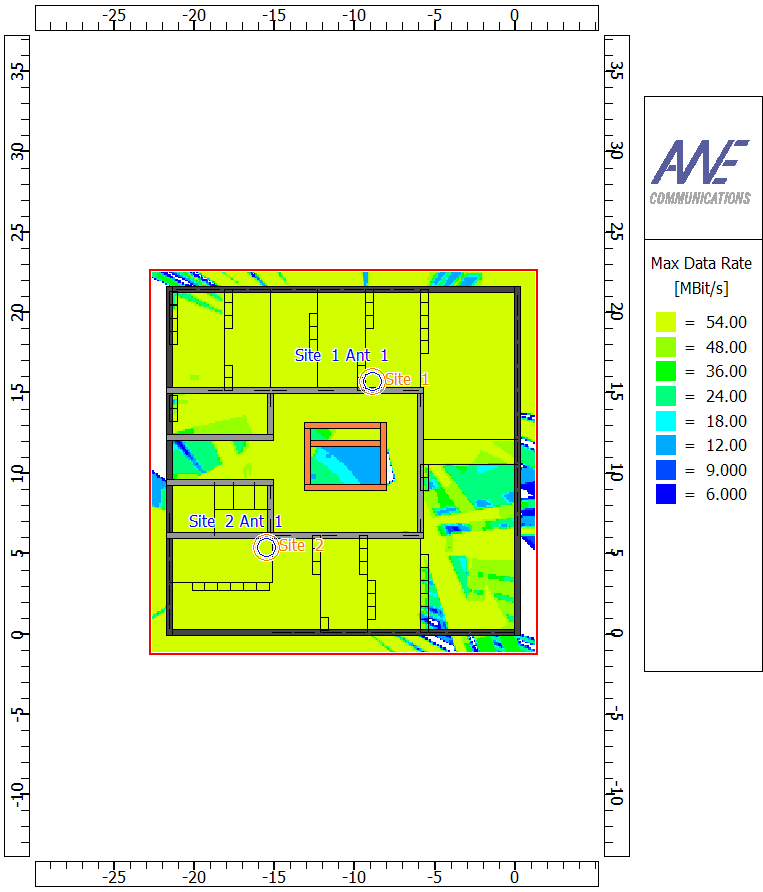
\includegraphics[scale=0.65]{RATE.png}
\end{figure}
\clearpage
\section{Zestawienie wyniku symulacji z obliczeniami własnymi}
\begin{figure}[h]
\centering
\caption{Symulacja i obliczenia własne - Multi-Wall Model}
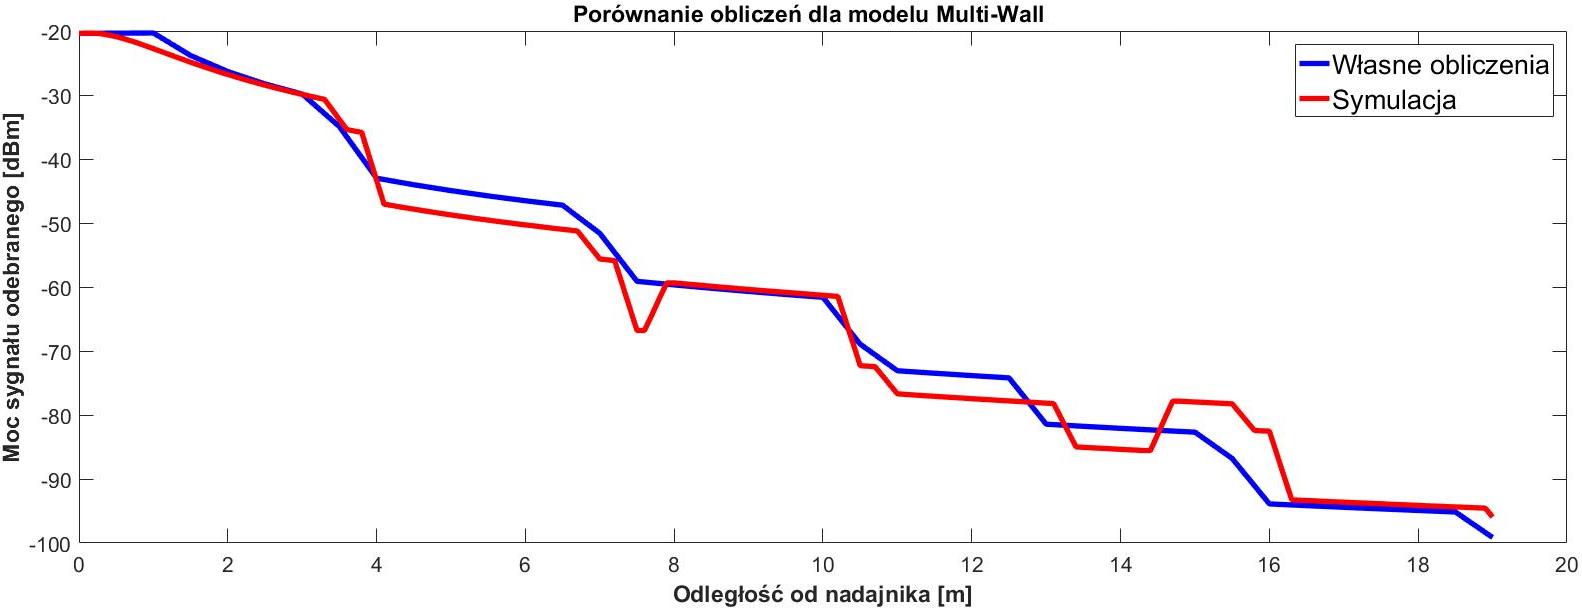
\includegraphics[scale=0.4]{comparation.png}
\end{figure}
\begin{figure}[h]
\centering
\caption{Symulacja i obliczenia własne - One-Slope Model ze współczynnikiem n = 2}
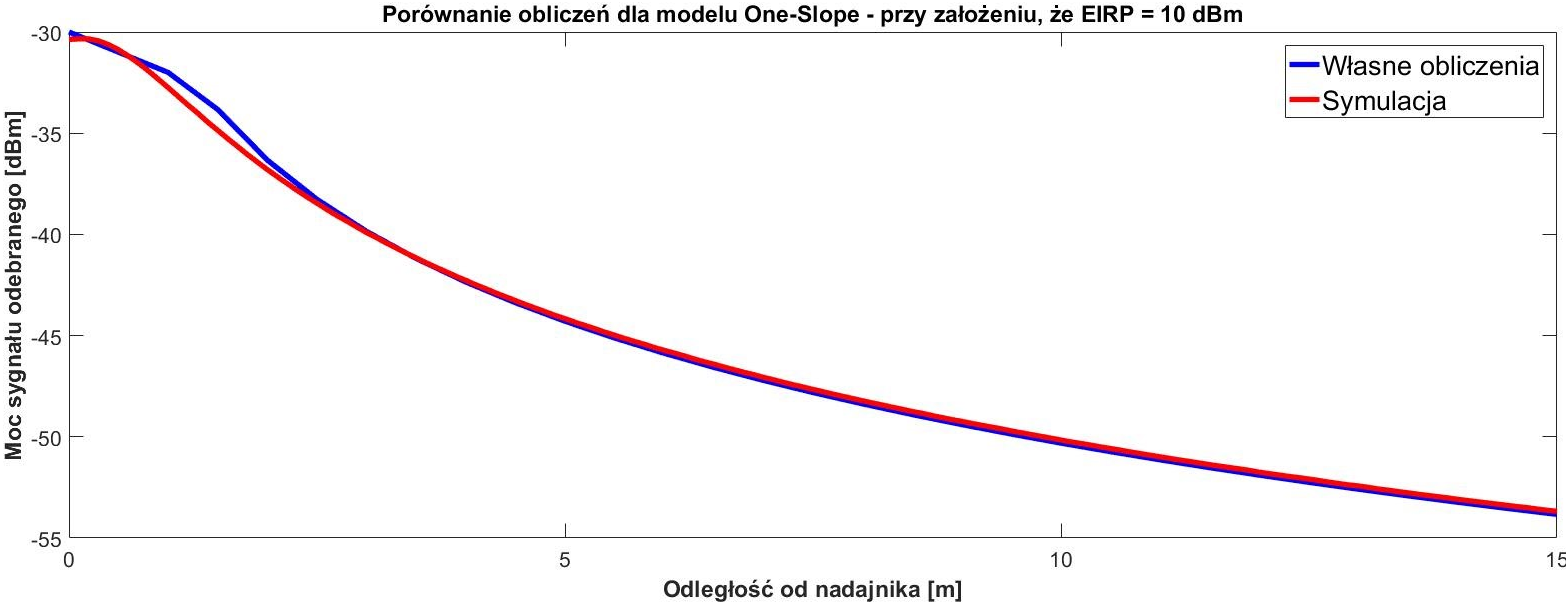
\includegraphics[scale=0.3]{comparation2.png}
\end{figure}
\clearpage
\section{Wnioski}
\indent\indent Porównując modele DPM, MWM oraz OSM zauważamy znaczne różnice przede wszystkim w~obszarze za silnie tłumiącą windą.\\

\indent DPM dzięki analizie odbić potrafi określić rozkład pola także za windą, co czyni go najdokładniejszym z analizowanych modeli. Takie podejście najlepiej przybliża zachowanie się fali EM w~rzeczywistym środowisku propagacyjnym. W tym modelu największą przeszkodę stanowią ściany otaczające windę, w której poziom odbieranego sygnału spada poniżej -100 dBm, co w przypadku większości odbiorników jest zbyt mało, aby wykryć sygnał.\\

\indent MWM analizuje jedynie prostą łączącą każdy punkt mapy z nadajnikiem, co powoduje, że punkty za zbrojoną ścianą, która otacza windę, nie otrzymują sygnału na poziomie, który umożliwiałby prowadzenie transmisji.\\

\indent W trakcie wykonywania ręcznych obliczeń dla modelu One-Slope okazało się, że po awarii programu najprawdopodobniej została ustawiona zła wartość EIRP dla nadajnika. Można to zauważyć, ponieważ dla każdego punktu na rysunku 13, krzywa przedstawiająca wynik symulacji jest obniżona o 10 dBm, co odpowiada ustawieniu EIRP = 10 dBm, czyli 10 dBm mniej niż zakładany poziom.\\

\indent OSM jest modelem, który w ogóle nie uwzględnia wnętrza budynku, tj. ścian, przeszkód w~postaci mebli, etc. Nie jest on modelem miarodajnym przy dokładnych obliczeniach, a~pozwala jedynie na pewne szacowanie tłumienia w~otoczeniu nadajnika. Prawdopodobnie lepiej sprawdziłby się w~dużych pomieszczeniach, jak np. hale produkcyjne, jednak w testowanym modelu budynku jest on zbyt mało dokładny. Jednocześnie porównując model OSM z pozostałymi dwoma (uwzględniając, że ustawiono złe EIRP), można zauważyć, że przyjmując n = 2 otrzymano wyniki zbyt pesymistyczne względem DPM oraz MWM - w bliskim otoczeniu i zbyt optymistyczne w porównaniu do MWM - dla dalszych obszarów. Przy n = 6 wyniki są zbyt pesymistyczne w porównaniu zarówno z DPM, jak i MWM.\\

\indent Dla dwóch punktów dostępowych, wykorzystując MWM do przeprowadzenia symulacji, uzyskano około 90\% pokrycia terenu szybkością transferu 54 MBit/s i blisko 100\% pokrycia terenu z~
szybkością transferu~$\geq$~18~MBit/s, co było pożądane w tym ćwiczeniu, a także pozwala na komfortową, dla użytkownika systemu, transmisję danych. Większość terenu pokryta jest mocą $\geq$ -70 dBm.
\clearpage
\section{Literatura}
\begin{enumerate}
\item Łukasz Jasiński, „Analiza i~porównanie modeli propagacyjnych dla środowiska wewnątrzbudynkowego”, Wrocław, 2011
\item Gerd Wölfle, René Wahl, Pascal Wildbolz, Friedrich Landstorfer,  „Dominant Path Prediction Model for Indoor Scenarios”, GeMiC, 2005
\end{enumerate}
\end{document}